% !TEX encoding = UTF-8 Unicode

\documentclass[a4paper,12pt]{article}
\usepackage[swedish]{babel}
\usepackage[utf8]{inputenc}
\usepackage{graphicx}
\usepackage{epstopdf}
\usepackage{gensymb}
%% Definitioner för LIPS-dokument

\usepackage[swedish]{babel}
\usepackage[utf8]{inputenc}
\usepackage[T1]{fontenc}
\usepackage{times}
\usepackage{ifthen}

\usepackage[margin=25mm]{geometry}

\usepackage{fancyhdr}
\pagestyle{fancy}
\lhead{}
\chead{\textbf{\LIPSprojekttitel}}
\rhead{\textbf{\textsl{LiTH}}\\\textbf{\LIPSdatum}}
\lfoot{\textbf{\LIPSkursnamn}\\\textbf{\LIPSdokumentansvarig}}
\cfoot{\textbf{\LIPSprojektgrupp}\\\textbf{\LIPSgruppepost}}
\rfoot{\textbf{\textsc{Lip}s}\\\textbf{Sida~\thepage}}

\setlength{\parindent}{0pt}
\setlength{\parskip}{1ex plus 0.5ex minus 0.2ex}


\newcommand{\twodigit}[1]{\ifthenelse{#1<10}{0}{}{#1}}
\newcommand{\dagensdatum}{\number\year-\twodigit{\number\month}-\twodigit{\number\day}}

%% ------------------------------------------
% NYBILD
% Skapar centrerad bild med caption
%   
% #1: Filens url relativt '/bilder/'
% #2:  Caption
% #3: Label
% #4: Skalning
%% ------------------------------------------
\newcommand{\nyBild}[4] 
{\begin{figure}[H]
  \centering
 \includegraphics[angle=0,scale=#4]{bilder/#1}
  \caption{#2}
  \label{fig:#3}
\end{figure}}



%%  Redefinitions of commands containing @
\makeatletter
\makeatother

\newcommand{\LIPStitelsida}{%
{\ }\vspace{45mm}
\begin{center}
  \textbf{\Huge \LIPSdokumenttyp}
\end{center}
\begin{center}
  {\Large Redaktör: \LIPSredaktor}
\end{center}
\begin{center}
  {\Large \textbf{Version \LIPSversion}}
\end{center}
\vfill
\begin{center}
  {\large Status}\\[1.5ex]
  \begin{tabular}{|*{3}{p{40mm}|}}
    \hline
    Granskad & \LIPSgranskare & \LIPSgranskatdatum \\
    \hline
    Godkänd & \LIPSgodkannare & \LIPSgodkantdatum \\
    \hline
  \end{tabular}
\end{center}
\newpage
}


\newenvironment{LIPSprojektidentitet}{%
{\ }\vspace{45mm}
\begin{center}
  {\Large PROJEKTIDENTITET}\\[0.5ex]
  {\small
  \LIPSartaltermin, \LIPSprojektgrupp\\
  Linköpings Tekniska Högskola, ISY
  }
\end{center}
\begin{center}
  {\small Gruppdeltagare}\\
%  \begin{tabular}{|p{30mm}|p{40mm}|p{35mm}|p{45mm}|}
  \begin{tabular}{|l|p{45mm}|p{25mm}|l|}
    \hline
    \textbf{Namn} & \textbf{Ansvar} & \textbf{Telefon} & \textbf{E-post} \\
    \hline
}%
{%
    \hline
  \end{tabular}
\end{center}
\begin{center}
  {\small
    \textbf{E-postlista för hela gruppen}: \LIPSgruppepost\\
    \textbf{Hemsida}: \LIPSgrupphemsida\\[1ex]
    \textbf{Kund}: \LIPSkund\\
    \textbf{Kontaktperson hos kund}: \LIPSkundkontakt\\
    \textbf{Kursansvarig}: \LIPSkursansvarig\\
    \textbf{Handledare}: \LIPShandledare\\
  }
\end{center}
\newpage
}
\newcommand{\LIPSgruppmedlem}[4]{\hline {#1} & {#2} & {#3} & {#4} \\}



\newenvironment{LIPSdokumenthistorik}{%
\begin{center}
  Dokumenthistorik\\[1ex]
  \begin{small}
    \begin{tabular}{|l|l|p{60mm}|l|l|}
      \hline
      \textbf{Version} & \textbf{Datum} & \textbf{Utförda förändringar} & \textbf{Utförda av} & \textbf{Granskad} \\
      }%
    {%
      \hline
    \end{tabular}
  \end{small}
\end{center}
}
\newcommand{\LIPSversionsinfo}[5]{\hline {#1} & {#2} & {#3} & {#4} & {#5} \\}

\newcounter{LIPSkravnummer}
\newcounter{LIPSunderkravnummer}[LIPSkravnummer]
\newenvironment{LIPSkravlista}{%
  \begin{tabular}{|p{25mm}|p{25mm}|p{85mm}|p{5mm}|}
    }%
  {%
    \hline
  \end{tabular}
}
\newcommand{\LIPSkrav}[3]{\hline\stepcounter{LIPSkravnummer}\textbf{Krav nr \arabic{LIPSkravnummer}} & \textbf{{#1}} & {#2} & \textbf{{#3}} \\}
\newcommand{\LIPSunderkrav}[3]{\hline\stepcounter{LIPSunderkravnummer}\textbf{Krav nr \arabic{LIPSkravnummer}\Alph{LIPSunderkravnummer}} & \textbf{{#1}} & {#2} & \textbf{{#3}} \\}





%%% Local Variables: 
%%% mode: latex
%%% TeX-master: "kravspec_mall"
%%% End: 



\newcommand{\LIPSartaltermin}{2012/VT}
\newcommand{\LIPSkursnamn}{TSEA27}

\newcommand{\LIPSprojekttitel}{Komborobot}

\newcommand{\LIPSprojektgrupp}{Grupp 17}
\newcommand{\LIPSgruppepost}{komborobot@googlegroups.com}
\newcommand{\LIPSgrupphemsida}{finns ej}

\newcommand{\LIPSdokumentansvarig}{Mattias Jansson}
\newcommand{\LIPSkund}{ISY, Linköpings universitet, 581\ 83 Linköping}
\newcommand{\LIPSkundkontakt}{Tomas Svensson, 013-281368, tomass@isy.liu.se}
\newcommand{\LIPSkursansvarig}{Tomas Svensson, 013-281368, tomass@isy.liu.se}
\newcommand{\LIPShandledare}{}


\newcommand{\LIPSdokumenttyp}{Banspecifikation}
\newcommand{\LIPSredaktor}{Simon Larsson}
\newcommand{\LIPSversion}{1.1}
\newcommand{\LIPSdatum}{\dagensdatum}

% Förslag till versionshantering:
% döp helt enkelt om filen till [dokument]_vX.Y.tex vid varje revision


\newcommand{\LIPSgranskare}{}
\newcommand{\LIPSgranskatdatum}{}
\newcommand{\LIPSgodkannare}{}
\newcommand{\LIPSgodkantdatum}{}

\begin{document}

\LIPStitelsida

%% Argument till \LIPSgruppmedlem: namn, roll i gruppen, telefonnummer, epost
\begin{LIPSprojektidentitet}
  \LIPSgruppmedlem{Simon Larsson}{Projektledare (PL)}{070-7311646}{simla804@student.liu.se}
  \LIPSgruppmedlem{\LIPSdokumentansvarig}{Dokumentansvarig (DOK)}{073-6837074}{matja307@student.liu.se}
  \LIPSgruppmedlem{Gustav Svensk}{Reglersystem (REG)}{073-6208776}{gussv666@student.liu.se}
  \LIPSgruppmedlem{Johan Jönsson}{Mjukvara (KA)}{073-8305758}{johjo939@student.liu.se}
  \LIPSgruppmedlem{Tobias Andersson}{Hårdvara (HV)}{073-7201098}{toban963@student.liu.se}
  \LIPSgruppmedlem{Markus Falck}{Leveransansvarig (LV)}{076-3457552}{marlo265@student.liu.se}
  \LIPSgruppmedlem{Simon Wallin}{Testansvarig (GM)}{076-2300665}{simwa252@student.liu.se}
\end{LIPSprojektidentitet}

\tableofcontents{}

\newpage

%% Argument till \LIPSversionsinfo: versionsnummer, datum, ändringar, utfört av, granskat av
\addcontentsline{toc}{section}{Dokumenthistorik}
\begin{LIPSdokumenthistorik}
\LIPSversionsinfo{1.0}{2012-01-31}{Första versionen}{gussv666}{johjo939}
\LIPSversionsinfo{1.1}{2012-05-11}{4-vägskorsningar är borttagna. Övergångar mellan linje/labyrint är uppdaterade}{simwa252}{simla804}

\end{LIPSdokumenthistorik}

\newpage

\section{Banspecifikation} 

Banan består av två huvuddelar: Linjedelar och labyrintdelar, där linjerna fungerar som transportsträcka till, från eller mellan en eller flera labyrinter. Linjen tar vid i mitten av labyrintgången 5 cm in i labyrinten där den slutar eller börjar. Labyrintens beståndsdelar varierar utifrån vilken prioritetsnivå som är uppfylld. Tävlingsdeltagarna kommer innan tävlingen överens om vilken av nivåerna som ska användas.
\\
\\
Linjedelen:
\\
Linjerna i banan skall bestå av en svart tejp på grått underlag. Tejpens bredd ska vara mellan 14-18 mm. I de fall en tjock linje nämns avses en tejplinje med bredd mellan 42-54 mm (tre tejpbredder). Med en smal tejplinje avses en linje med bredd 14-18 mm (en tjepbredd). Tejpbanan kan korsa sig själv i 90\degree korsningar, den kan dock ej dela sig. Svängradien för banan är minst 25 cm. Banan avslutas med en stoppsignal eller övergår till en labyrint. Stoppsignalen inleds med en 30 cm raksträcka som sedan övergår i en tvärgående linje följt av tre parallella smala linjer, 1 tejbredd isär med mitten där den tidigare linjen avslutades, i färdriktningen. Banan kan endast avslutas i linje läge och aldrig i en labyrint. När banan övergår till linje från labyrint så görs det med två linjer som 20 cm från kanten in mot mitten. Linjerna går sedan ihop i en linje efter 30 cm. Tjeplinjen ska vid, övergång till labyrint gå in rakt mitt mellan väggarna och fortsätta 10 cm rakt in i labyrinten. För samtliga mått och placeringar se Figur \ref{fig:labyrintanvisningar}.
\\


Labyrintdelen:

\begin{list}{*}{}
\item Nivå 1: Avståndet mellan parallella väggar är 80 cm. 3-vägskorsningar kan förekomma, dock med räta vinklar mellan varandra, rätt väg anges av markeringar på golvet. Markeringarna görs med två linjer som går vinkelrätt mellan väggarna. En tjock linje följd av en tunn indikerar höger, en tunn följd av en tjock indikerar vänster och två linjer av samma tjocklek rakt fram. Markeringarna ska vara 50 cm breda och liga 15 cm från vardera sida av labyrinten. En raksträcka på 25 cm ska följa fram till korsningen. 
\item Nivå 2: Som nivå 1 med följande justeringar: Inga markeringar behövs då ena vägen vid en korsning är en återvändsgränd med djup på 80 cm.
\item Nivå 3: Som nivå 1 med följande justeringar: Inga markeringar nödvändiga. Hål 80 cm stora ut ur labyrinten som inte leder någonstans kan förekomma.
\end{list} 

\begin{figure}[h!]
	
	\begin{center}
		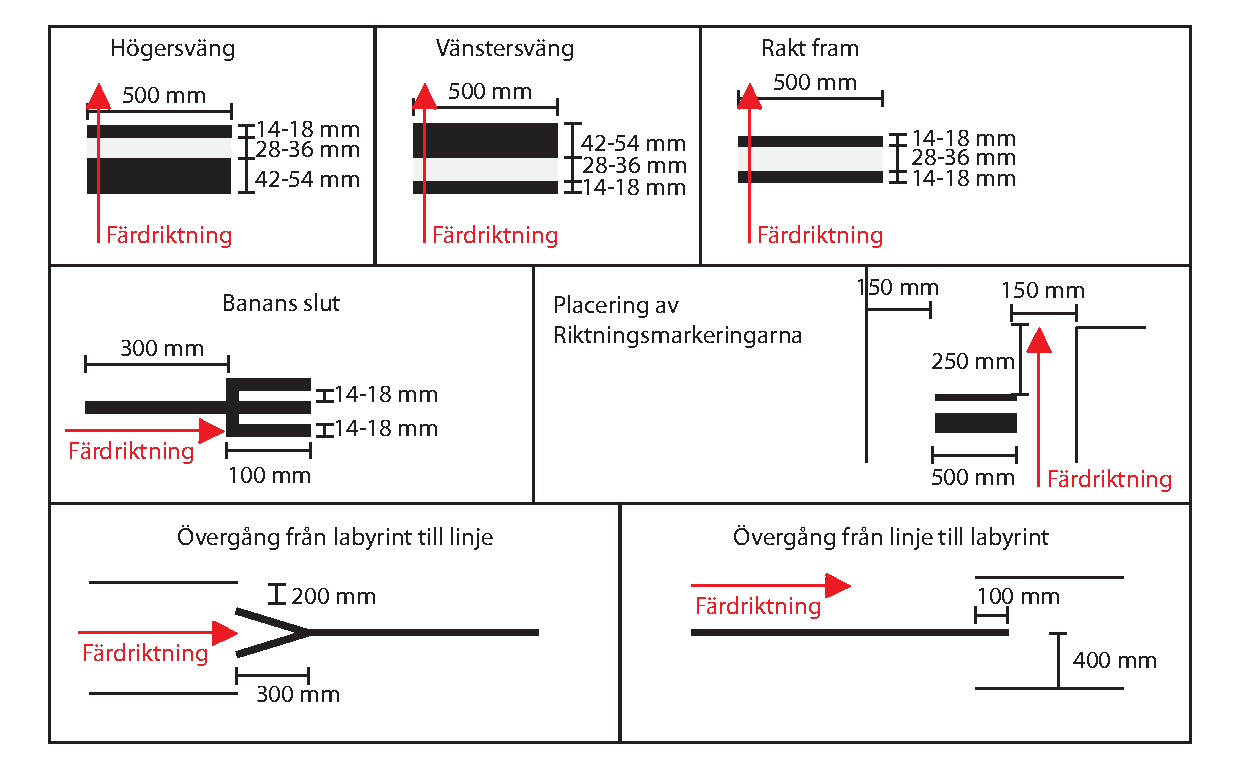
\includegraphics[scale=0.8,angle=0]{Labyrintanvisningar.pdf}
	\end{center}
	\caption{Mått till labyrintanvisningar}
	\label{fig:labyrintanvisningar}
\end{figure}

\end{document} 


%%% Local Variables: 
%%% mode: latex
%%% TeX-master: t
%%% End: 
